%% -*- coding: utf-8; -*-

%% \listfiles

\documentclass[
  dissertacao,
  brazil
]{ThesisPUC}

  %% \usepackage[brazilian]{babel}      %% in ThesisPUC.cls
  %% \usepackage[utf8]{inputenc}        %% .
  %% \usepackage[T1]{fontenc}           %% .
  %% \usepackage{lmodern}               %% .
  %% \usepackage[pdftex]{graphicx}	%% .

  \usepackage{tabularx}
  \usepackage{multirow}
  \usepackage{multicol}
  \usepackage{colortbl}
  \usepackage[%
    dvipsnames,
    svgnames,
    x11names,
    fixpdftex
  ]{xcolor}
  \usepackage{numprint}
  \usepackage{textcomp}
  \usepackage{booktabs}
  \usepackage[final]{pdfpages}
  
  %pacotes para as tabelas
  \usepackage[table,xcdraw]{xcolor}
  \usepackage{adjustbox}
  
  \usepackage{amsmath}
  \usepackage{enumitem}
  \usepackage{amssymb}
  \usepackage{textcomp}



%%% Other commands

\newcommand{\Rset}{\mathbb{R}}
\newcommand{\Zset}{\mathbb{Z}}

\npthousandsep{}
\npdecimalsign{,}

\modotabelas{figtab} %% [nada, fig, tab ou figtab]

\setcounter{tocdepth}{3}
\setcounter{secnumdepth}{3}


%%%
%%% My files
%%%

% -*- coding: iso-8859-1; -*-

\newcommand{\degree}{\ensuremath{^\circ}}

\newcommand{\cetem}{Centro de Tecnologia Mineral}

%\newcommand{\cetem@ini}{CETEM}
%\newcommand{\ini}[1]{\renewcommand{\cetem@ini}{#1}}
\newcommand{\CETEM}{CETEM}


%%%
%%%
%%%
\newcommand{\mybulletOB}{%
  % \textbullet
  % \checkmark
  $\triangleright$
  %\textopenbullet
}

\newcolumntype{L}{>{\raggedright \arraybackslash}X}
\newcolumntype{R}{>{\raggedleft \arraybackslash}X}
\newcolumntype{C}{>{\centering \arraybackslash}X}
\newcolumntype{M}[1]{>{\centering\hspace{0pt}}m{#1}}

\newcommand{\mrcel}[2]{%
\begin{tabular}[c]{@{}c@{}}#1\\#2\end{tabular}}

\newcommand{\mrcell}[2]{%
\begin{tabular}[l]{@{}l@{}}#1\\#2\end{tabular}}

\newcommand{\mrcelthree}[3]{%
\begin{tabular}[c]{@{}c@{}c@{}}#1\\#2\\#3\end{tabular}}

\newcommand{\mrcelcolorg}[2]{%
\begin{tabular}{l}\rowcolor{Gainsboro}#1\\#2\end{tabular}}

\newcommand{\tbthreeblabla}[3]{%
\begin{tabular}{ l @{\extracolsep{2mm}}X }
  \mybulletOB #1
  \mybulletOB #2
  \mybulletOB #3
\end{tabular}}

\newcommand{\mytbcimg}[3]{%
  \multicolumn{1}{C}{\parbox[c]{#1}{\includegraphics[width=#2]{#3}}}}

%%%
%%% In table-2.1
%%%

\newcommand{\colmund}[1]{\npmakebox[abcdef][c]{#1\degree}}


%%%
%%% Titulos
%%%

\tituloglossario{Lista de Abreviaturas}

\autor{Rodrigo Leite da Silva}
\autorR{Leite da Silva, Rodrigo}

\orientador{Edward Hermann Haeusler}{Prof.}
\orientadorR{Hermann Haeusler, Edward}

%\coorientador{}{}
%\coorientadorR{}
%\coorientadorInst{}{}

\titulo{Transcrição Automática de Pandeiro para Partitura}

%% \subtitulo{Subtitulo}

\dia{27}
\mes{Novembro}
\ano{2019}

\cidade{Rio de Janeiro}
\CDD{620.11}
\departamento{Informática}
\programa{Engenharia de Computação}
\centro{Centro Técnico Científico}
\universidade{Pontifícia Universidade Católica do Rio de Janeiro}
\uni{PUC-Rio}


%%%
%%% Banca
%%%

\banca{%
%  \membrodabanca{Nome}{Prof.}
%    {Pontifícia Universidade Católica do Rio de Janeiro}{PUC-Rio}
%  \membrodabanca{Nome}{Prof.}
%    {Pontifícia Universidade Católica do Rio de Janeiro}{PUC-Rio}
}


%%%
%%% Currículo
%%%

\curriculo{}



%%%
%%% Agradecimentos
%%%

\agradecimentos{}


%%%
%%% Prechaves
%%%

\catalogprekeywords{%
  \catalogprekey{}%
}


%%%
%%% Chaves
%%%

\chaves{%
  \chave{}
}


%%%
%%% Resumo
%%%

\resumo{}


%%%
%%% Epigrafe
%%%

%% \epigrafe{%
%%   no epigrafe}
%% \epigrafeautor{}
%% \epigrafelivro{}


%%%
%%% Misc.
%%%

\usecolour{true}


%%%
%%% 
%%%


\begin{document}

\selectlanguage{brazilian}

\chapter{Introdução}
\section{Transcrição Automática de Música}
Transcrever uma música é o ato de escutá-la e escrever, em notação musical (e.g.: partituras pautadas), as notas que a compõem \cite{martin1996blackboard}. A automatização consiste em usar uma máquina para realizar esse processo que, para humanos, requer um grau de educação musical crescente proporcional à complexidade da música.

A \tam s (daqui em diante \TAM) tem muitos usos possíveis sendo, o mais evidente, a gravação das notas de uma performance improvisada. São outros usos para \TAM: registro de músicas em estilos onde o improviso é parte íntegra da execução; busca e anotação automática de músicas; sistemas interativos de música; além de análise musicológica \cite{benetos2013automatic}.

Para sinais monofônicos (i.e.: um único instrumento) o problema é considerado praticamente resolvido com \cite{klapuri1998automatic} e os trabalhos atuais são mais voltados para sinais polifônicos. Entretanto, comparado a trabalhos focados em instrumentos harmônicos, são poucos os feitos com instrumentos percussivos não-harmônicos em mente e, desses trabalhos, a maior parte é voltada para a bateria. 

\section{Motivação}

Na cultura brasileira, instrumentos percussivos são tão variados quanto ubíquos, graças ao sincretismo das culturas indígenas, africanas e européias. E, dentre esses instrumentos, o pandeiro tem uma versatilidade enorme, sendo normalmente usado do choro a MPB, mas com potencial em qualquer ritmo, graças à variedade de timbres que dele podemos extrair \cite{magalhaes2016pandeiro}. Essa variedade de abordagens, pareada com o baixo custo e portabilidade do instrumento, torna-o um ótimo ponto de entrada para o mundo da percussão. 

Visando aproximar os trabalhos já realizados de \TAM \space para o contexto musical brasileiro propomos, nessa monografia, um sistema que faça a transcrição automática do pandeiro para uma partitura pautada.


\section{Ambiente Computacional}
A linguagem escolhida para implementação do sistema proposto foi Python \cite{van2011python}, por ter a maior variedade de bibliotecas de \mir \space (daqui em diante \MIR).

Querendo que o desempenho do editor não dependa da máquina onde o autor se encontra escolhemos, para desenvolvimento em Python, o Google Colab, um ambiente Jupyter Notebook \cite{kluyver2016jupyter}, para criação e edição de documentos que mesclam texto e código interativo. O Colab roda completamente na nuvem eliminando a necessidade da configuração de um ambiente local. A natureza interativa dos documentos criados facilitam a reprodução do trabalho e a iteração ágil no desenvolvimento de trechos de código.

Foi escolhida Essentia como a biblioteca de \MIR \space para nosso sistema ao invés da LibROSA, pois dispõe dos modos \emph{standard}, onde podemos testar algoritmos rapidamente, e \emph{streaming}, onde podemos declarar um novo algoritmo como uma rede de outros algoritmos, facilitando a declaração de uma arquitetura para nosso sistema. Essentia também dispõe de muitos tutoriais para suas funcionalidades em formato Jupyter Notebook (.ipynb), facilitando seu aprendizado.

\chapter{Situação Atual}

Encontramos os seguintes trabalhos focados na \TAM \space monofônicas de percussão não-harmônica. Schloss \cite{schloss1986automatic} construiu um sistema capaz de transcrever improvisos numa Conga para uma partitura pautada modificada. Para a Tabla, um instrumento do norte da Índia, Chordia \cite{chordia2005segmentation} implementou um sistema que segmenta um áudio do instrumento em suas notas e as classifica, enquanto Gillet e Richard \cite{gillet2003automatic} fizeram um ambiente inteiro (Tablascope) que permite a transcrição automática em tempo real para notação de Tabla, edição de frases, anotação de áudio, além de outras funcionalidades. Sillanpää \cite{sillanpaa2000drum} trabalhou sobre a bateria, com o objetivo de identificar até três toques simultâneos. Anantapadmanabhan, Bellur e Murthy \cite{anantapadmanabhan2013modal} analisaram os toques do Mridangam, um instrumento do sul da Índia, e estenderam a análise para ensinar um \hmm \space (\HMM) a transcrever o instrumento. 

Trabalhos voltados para o aspecto rítmico de \TAM \space foram. Takeda, Nishimoto e Sagayama \cite{takeda2007rhythm} que, inspirados em trabalhos de reconhecimento de fala, treinaram um \HMM\space a reconhecer um "vocabulário rítmico" e, subsequentemente, estimaram o ritmo e andamento de uma música em formato MIDI.
Guaus e Herrera \cite{guaus2005rhythm}, trabalhando no contexto de classificação de gênero musical, definiram e implementaram uma "Transformada Rítmica". Essa transformada serve para representar de maneira genérica o ritmo da música, análogo a como a Transformada de Fourrier representa timbre.


\section{Tecnologias Existentes}
Essentia \cite{bogdanov2013essentia}, LibROSA \cite{mcfee2015librosaDesign} e mir\_eval \cite{raffel2014mir_eval} são bibliotecas desenvolvidas para \MIR. Essentia, escrito em C++ com envoltório em Python, fornece diversos algoritmos de análise de sinal em dois modos: \emph{standard} e \emph{streaming}, usados de modo imperativo e declarativo, respectivamente. LibROSA, foi escrito em Python e fornece análises de sinais musicais tanto de baixo nível (onsets, andamento) quanto de alto nível (estrutura da música). mir\_eval, por sua vez, fornece medidas de desempenho para diversas tarefas de \MIR.

music21 \cite{cuthbert2010music21}, é uma biblioteca desenvolvida analisar e sintetizar músicas, através de suas representações (i.e. partituras).

MusicXML \cite{good2001musicxml} é um formato de arquivo que se propõe a ser o formato que representa a notação musical ocidental de maneira intercambiável entre aplicações de notação musical, análise musical etc.

\section{Conceitos Relevantes}
\begin{itemize}
    \item Andamento: O pulso regular, medido em batidas por minuto, que guia a música.
    \item Ritmo: Como os toques estão organizados dentro do andamento.
\end{itemize}



\chapter{Objetivos do Trabalho}
A proposta do projeto é implementar um sistema que receba um arquivo de áudio de pandeiro e retorne uma representação em partitura pautada. Dividido, a grosso modo, em três etapas consecutivas: segmentação do sinal e reconhecimento das respectivas notas; extração de informações rítmicas do sinal; escrita da partitura.

Para cada uma dessas etapas, estudamos tecnologias que já foram usadas em outros trabalhos, avaliando suas respectivas viabilidades para projeto proposto. Encontramos bibliotecas que atendem aos requisitos de cada uma das etapas. Todas elas usadas em Python. 

Queremos atender a qualquer usuário com um pandeiro, microfone e editor de partituras. Uma interface gráfica não está prevista no projeto mas a partitura resultante do sistema deverá estar em algum formato editável por programas corriqueiros. Essa facilidade de edição é vital para que os usuários validem o resultado do sistema e corrijam quaisquer equívocos na transcrição.

Durante a pesquisa, determinamos que precisaremos constuir um conjunto de dados não rotulado de toques do pandeiro. Esse conjunto será usado por algoritmos de agrupamento para encontrar grupos de toques semelhantes.

\section{O Sistema}
\subsection{Particularidades do Pandeiro Brasileiro}
Algumas particularidades do instrumento em questão, que estão sendo consideradas no projeto do sistema: 
\begin{itemize}
    \item O sinal será monofônico (apenas um pandeiro), então não estamos preocupados com a identificação e separação de múltiplos instrumentos presentes.
    \item Por ser sustentado com uma mão e atacado com outra, não ocorrem toques simultâneos. As soalhas (platinelas) soam em todos os toques, mas os toques agudos podem ser caracterizados pela ausência de um ataque na pele.
\end{itemize}

\subsection{Segmentação e Extração de \emph{Features}}
Vou usar a biblioteca Essentia para encontrar o \emph{onset} dos toques e extrair \emph{features} do sinal para a tarefa de reconhecer os toques.

\subsection{Reconhecimento dos Toques}
Pela falta de um conjunto de dados rotulados de toques de pandeiro, optamos por usar aprendizado de máquina não-supervisionado. Para essa tarefa de classificação de toques, algoritmos de agrupamento são os mais apropriados, e a biblioteca Scikit-Learn oferece implementações de vários desses \cite{scikit2019Clustering}.

Como alguns dos toques são, executados com a intenção de soarem identicos para o ouvido humano (e.g. o grave de polegar e o grave de bloco de dedos), esperamos ter dificuldade nas suas classificações.

\subsection{Reconhecimento de Andamento}
Na biblioteca Essentia já existem algoritmos de identificação da assinatura de batidas por minuto.

\subsection{Reconhecimento de Ritmo}
Essentia tem uma implementação da Rhythm Transform, entretanto, no manual do algoritmo, informa que a qualidade não é garantida:
\begin{quote}
    Quality: experimental (non-reliable, poor accuracy according to tests on simple loops, more tests are necessary).
\end{quote}

\subsection{A partitura resultante}
Por ser um instrumento não-harmônico, a notação típica em pentagramas (cinco linhas), onde a posição da nota reflete a frequência do som emitido pelo instrumento, não é útil. Seuguirei então o trabalho de Magalhães \cite{magalhaes2018tecnica}, que definiu uma \CA (ou \ca) para o pandeiro brasileiro, ou seja, um indicador do que cada linha e espaço significa. Isso reduz a quantidade de linhas necessárias de cinco (pentagrama) para duas (bigramas). Então usaremos a mesma \ca que Magalhães e as 9 notas do pandeiro como definido por ela.

A partitura será representada em formato MusicXML, que será gerado através da biblioteca music21, que disponibiliza uma função específicamente para a essa tarefa.

\begin{figure}
    \centering
    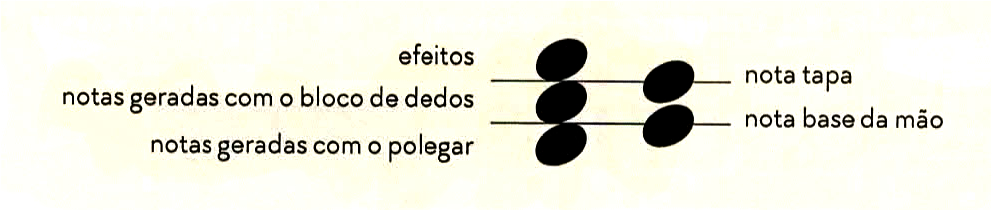
\includegraphics[width=\textwidth]{ClaveDeArticulacao.jpg}
    \caption{Clave de articulação usada nas partituras}
    \label{fig:clave}
\end{figure}


\chapter{Revisão do Plano de Ação}
\section{O plano original}
O plano de ação prevê ciclos de pesquisa e desenvolvimento menores e mais frequentes, que construam o sistema de forma gradual.
Ambos períodos de pesquisa e implementação dão divididos nas partes referentes a: extração das notas do sinal (quais são e quando foram tocadas); extração de informações rítmicas (tempo, métrica, andamento); tradução da informação coletada para uma partitura.

A criação de dados de aprendizado e teste foi incluída no cronograma pelo motivo já mencionado e pretendemos coletar sons provenientes de pandeiros com variação nos materiais( da membrana, das platinelas, do corpo) e nos diâmetros.


\section{Dificuldades e Pendências}

O único aspecto proposto pelo plano que não foi realizado foi a criação dos conjuntos de dados.
Isso foi deliberado durante o decorrer da pesquisa, pois notamos que montar conjuntos de dados anotados seria, por diversos motivos, muito trabalhoso.
A diversidade de pandeiros, com tamanhos e materiais diferentes, é muito grande. 
Portanto, para a coleta de dados suficentes para ensinarmos uma máquina a aprender a reconhecer \emph{qualquer} pandeiro, precisaríamos de mais tempo do que o cronograma permite. 

Vamos limitar, então, o escopo do conjunto de dados de toques do pandeiro para apenas um instrumento: Um pandeiro de 11 polegadas, membrana de couro de cabra e platinelas de latão.
E julgamos que o conjunto de dados de várias notas formando um ritmo não será necessário. Não usaremos aprendizado de máquina para a etapa de identificação de ritmos.

\cronogramaoriginal
%\begin{wrapfigure}
%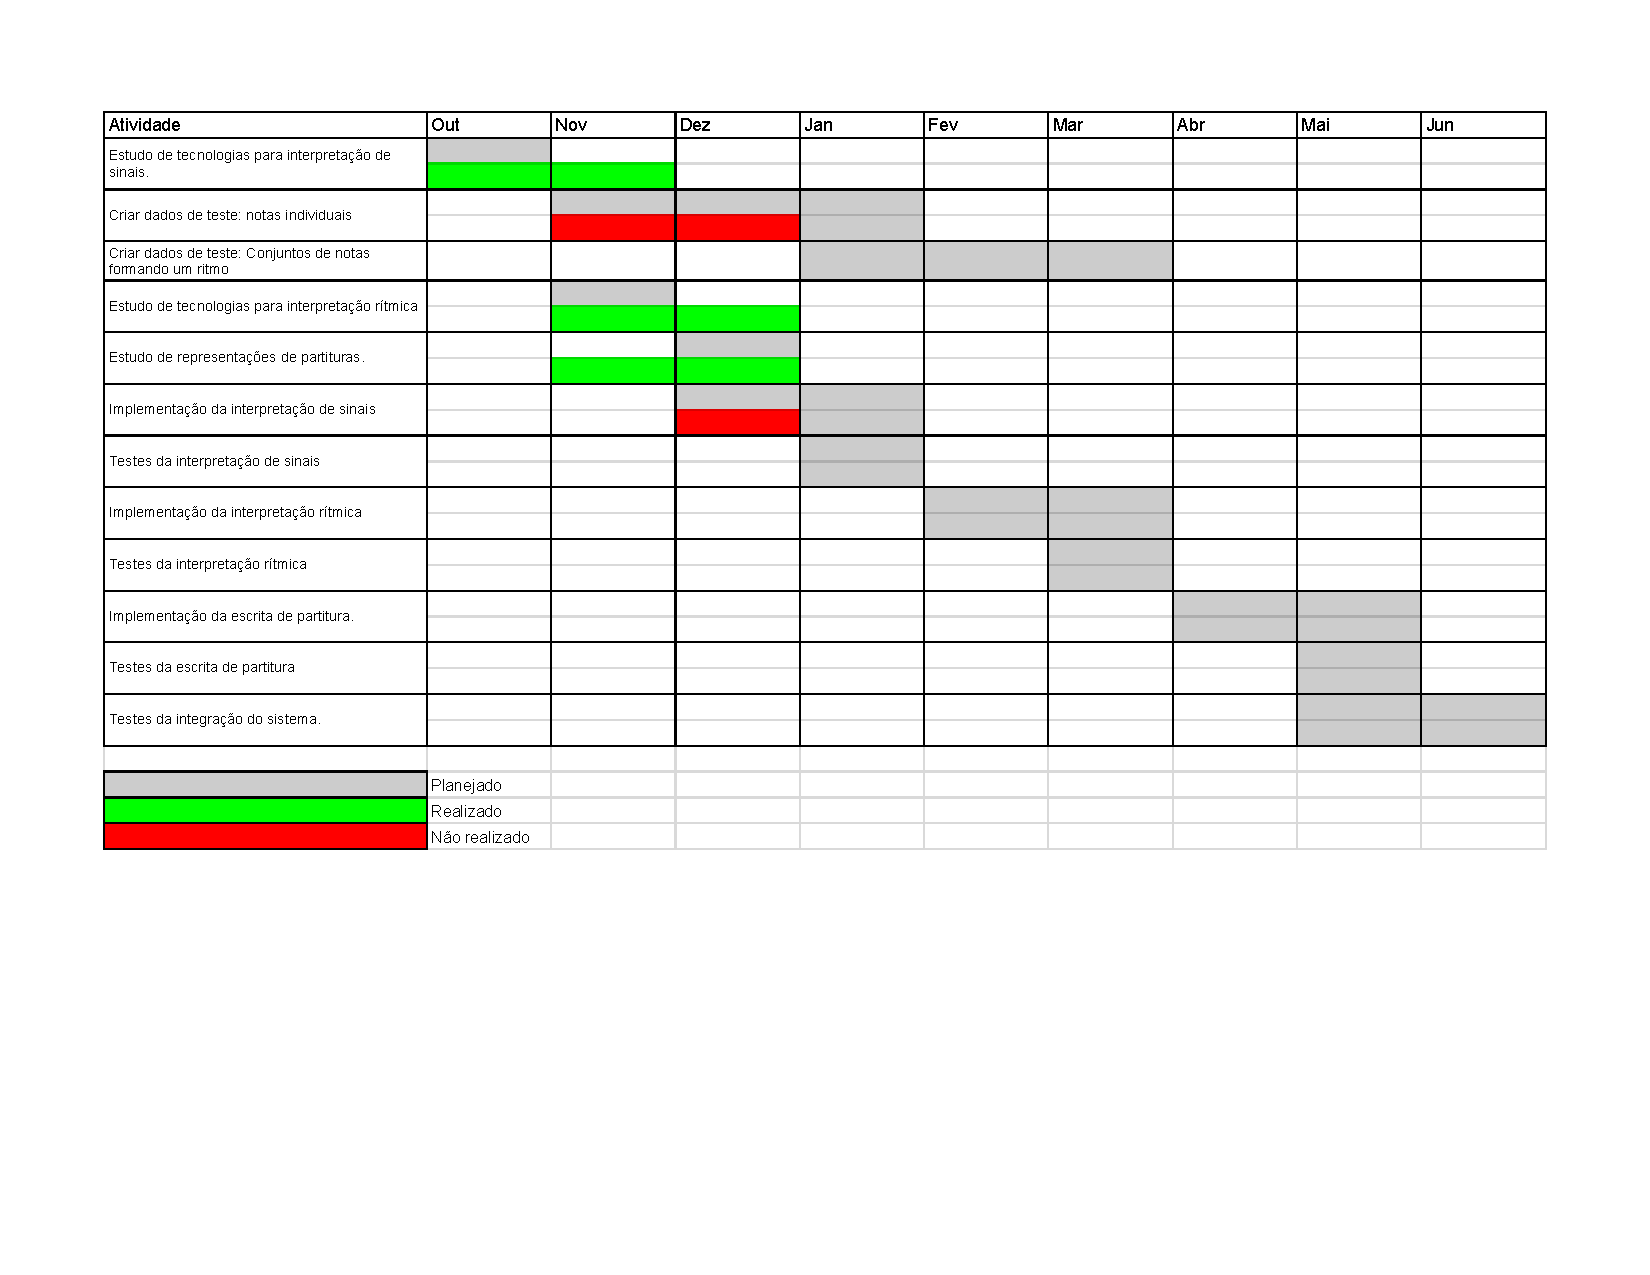
\includepdf{CronogramasReal.pdf}
%\end{wrapfigure}

\cronogramanovo
%\begin{wrapfigure}
%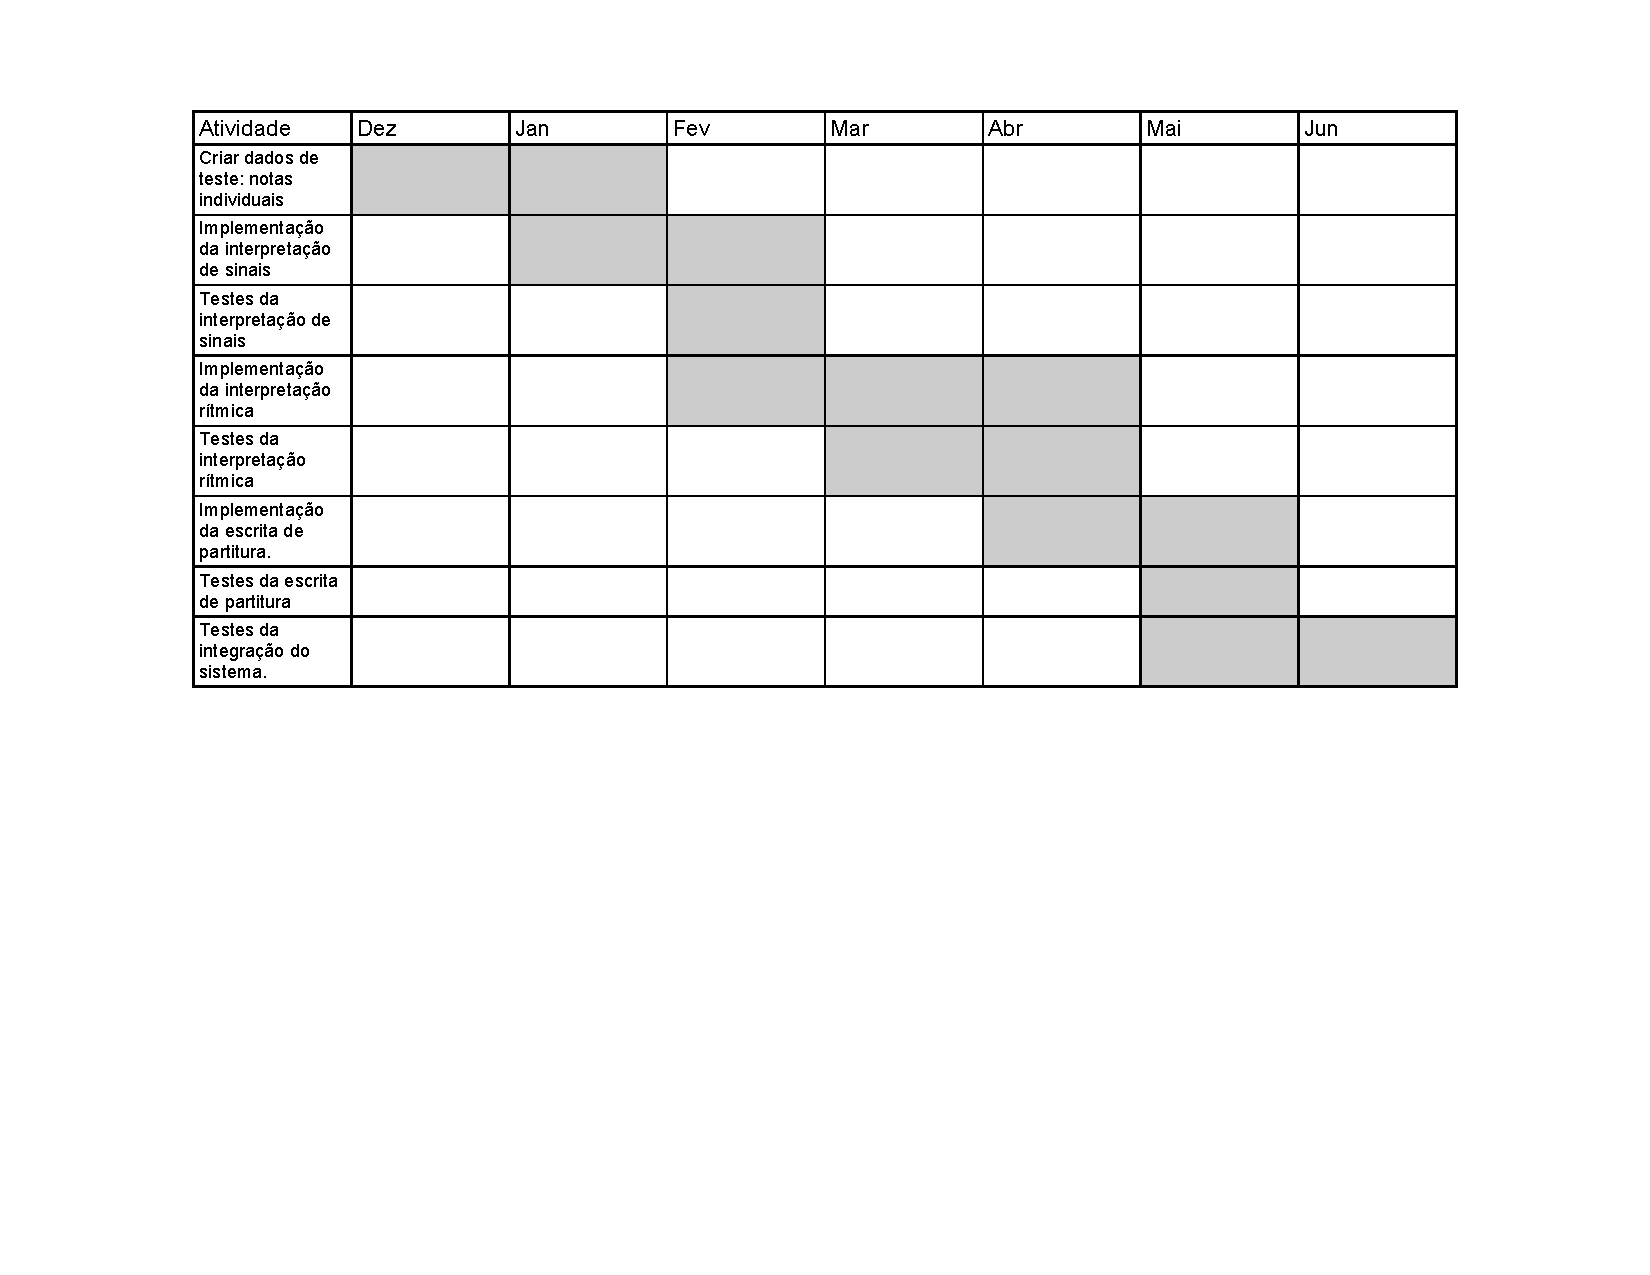
\includepdf{CronogramasFinal.pdf}
%\end{wrapfigure}

\arial
\bibliography{bibliografia}
\normalfont

\end{document}